\documentclass[10pt,a4paper]{article}
\usepackage[margin=2.2cm]{geometry}
\usepackage{fontspec,unicode-math}
\setmainfont{Libertinus Serif}\setsansfont{IBM Plex Sans}[Scale=0.9]\setmonofont{IBM Plex Mono}[Scale=0.85]
\setmathfont{Libertinus Math}
\usepackage{graphicx,booktabs,tabularx,multicol,xcolor,hyperref,enumitem}
\hypersetup{colorlinks,linkcolor=black,urlcolor=blue!50!black}
\newcommand{\ax}[1]{\par{\raggedright\noindent\hangindent=2.5em\hangafter=1 $#1$\par}\smallskip}
\setlength{\parindent}{0pt}\setlength{\parskip}{3pt}\setlength{\emergencystretch}{3em}
\newcommand{\tth}[1]{\texttt{#1}}
\title{Experiment concepts in description logic\\[2pt]\large with a partonomy, and the challenge-rescue experiment as an instance}
\author{Generated from \texttt{experiment\_concepts.ldl} by \texttt{rsa/experiment\_dl.py}}
\date{}
\begin{document}\maketitle
\section*{Conventions}
The concepts are stated in $\mathcal{SROIQ}(\mathbf{D})$, the logic of OWL~2~DL. Concept names are set in
$\mathsf{sans}$, role names in $\mathit{italics}$, individuals in $\mathtt{mono}$. A filler restriction
$(=\!n\;r.C)$ means exactly $n$ $r$-successors in $C$; $\exists r.C$ at least one; $\forall r.C$ only $C$.
Each LDL clause \texttt{(has \emph{role pattern cardinality})} becomes one number restriction,
\texttt{(only \emph{role pattern})} one value restriction, a pattern's slots nested existentials, and
\texttt{(role $x$)} the restriction $\exists\mathit{hasRole}.\mathsf{X\,Role}$.

Conformance of an experiment is checked under the \emph{closed-world} reading: the axioms are integrity
constraints over the instance as given, derived and placed (\texttt{rsa/experiment\_concepts.py}). An OWL reasoner
reads the same axioms under the open world: it would infer a missing culture rather than report it. Constraints that
$\mathcal{SROIQ}(\mathbf{D})$ cannot express are stated in Section~\ref{sec:beyond} in the logic they need.

\section{Roles and partonomy (RBox)}
Parthood ($\mathit{hasPart}$) is transitive and has four kinds: temporal parts of processes ($\mathit{hasPhase}$,
$\mathit{hasStep}$), material parts ($\mathit{hasWell}$) and components of plans and information entities
($\mathit{hasComponent}$: $\mathit{hasExposure}$, $\mathit{hasObservation}$, $\mathit{hasCandidate}$). Three relations
are deliberately \emph{not} parthood: a culture is \emph{contained in} a well (location), an action \emph{realizes} a
part of the plan, and a culture \emph{participates} in the actions it undergoes.

\begin{multicols}{2}
\ax{\mathit{hasPhase} ⊑ \mathit{hasPart}}
\ax{\mathit{hasStep} ⊑ \mathit{hasPart}}
\ax{\mathit{hasComponent} ⊑ \mathit{hasPart}}
\ax{\mathit{hasExposure} ⊑ \mathit{hasComponent}}
\ax{\mathit{hasObservation} ⊑ \mathit{hasComponent}}
\ax{\mathit{hasCandidate} ⊑ \mathit{hasComponent}}
\ax{\mathit{hasWell} ⊑ \mathit{hasPart}}
\ax{\mathit{hasUnit} ⊑ \mathit{hasParticipant}}
\ax{\mathit{hasCulture} ⊑ \mathit{hasUnit}}
\ax{\mathit{hasSubstance} ⊑ \mathit{hasParticipant}}
\ax{\mathit{hasSite} ⊑ \mathit{hasParticipant}}
\ax{\mathit{hasQuestion} ⊑ \mathit{specifies}}
\ax{\mathit{hasGoal} ⊑ \mathit{specifies}}
\ax{\mathit{hasSharedConditions} ⊑ \mathit{specifies}}
\ax{\mathit{hasComparison} ⊑ \mathit{specifies}}
\ax{\mathit{prevents} ⊑ \mathit{specifies}}
\ax{\mathit{maintains} ⊑ \mathit{specifies}}
\ax{\mathit{hasInsight} ⊑ \mathit{hasOutput}}
\ax{Trans(\mathit{hasPart})}
\ax{\mathit{partOf} ≡ \mathit{hasPart}^{-}}
\ax{\mathit{containedIn} ≡ \mathit{contains}^{-}}
\ax{\mathit{containedIn} ∘ \mathit{partOf} ⊑ \mathit{locatedIn}}
\ax{\mathit{hasPart} ∘ \mathit{hasParticipant} ⊑ \mathit{hasParticipant}}
\end{multicols}
OWL~2 allows number restrictions only on simple roles. Non-simple here: $\mathit{hasPart}$, $\mathit{hasParticipant}$, $\mathit{locatedIn}$, $\mathit{partOf}$. Roles in number restrictions: $\mathit{hasBelief}$, $\mathit{hasCandidate}$, $\mathit{hasComparison}$, $\mathit{contains}$, $\mathit{hasGoal}$, $\mathit{hasInsight}$, $\mathit{hasPhase}$, $\mathit{hasQuestion}$, $\mathit{hasSharedConditions}$, $\mathit{hasSite}$, $\mathit{hasSubstance}$, $\mathit{hasUnit}$. All are simple.
\section{Kinds and their partonomy}
Four disjoint kinds. Parthood never crosses kinds: a process has processes as parts, a plate has wells, a treatment has exposures, a question has candidate hypotheses.
\begin{multicols}{2}
\ax{\mathsf{Process} ⊓\allowbreak \mathsf{MaterialEntity} ⊑ ⊥}
\ax{\mathsf{Process} ⊓\allowbreak \mathsf{PlanSpecification} ⊑ ⊥}
\ax{\mathsf{Process} ⊓\allowbreak \mathsf{InformationEntity} ⊑ ⊥}
\ax{\mathsf{MaterialEntity} ⊓\allowbreak \mathsf{PlanSpecification} ⊑ ⊥}
\ax{\mathsf{MaterialEntity} ⊓\allowbreak \mathsf{InformationEntity} ⊑ ⊥}
\ax{\mathsf{PlanSpecification} ⊓\allowbreak \mathsf{InformationEntity} ⊑ ⊥}
\ax{\mathsf{Process} ⊑ ∀\mathit{hasPart}.\mathsf{Process}}
\ax{\mathsf{MaterialEntity} ⊑ ∀\mathit{hasPart}.\mathsf{MaterialEntity}}
\ax{\mathsf{PlanSpecification} ⊑ ∀\mathit{hasPart}.\mathsf{PlanSpecification}}
\ax{\mathsf{InformationEntity} ⊑ ∀\mathit{hasPart}.\mathsf{InformationEntity}}
\end{multicols}
\section{Entities}
\begin{multicols}{2}
\ax{\mathsf{Action} ⊑ \mathsf{Process}}
\ax{\mathsf{Culture} ⊑ \mathsf{MaterialEntity}}
\ax{\mathsf{Substance} ⊑ \mathsf{MaterialEntity}}
\ax{\mathsf{Plate} ⊑ \mathsf{MaterialEntity}}
\ax{\mathsf{Plate} ⊑ ∃\mathit{hasWell}.\mathsf{Well}}
\ax{\mathsf{Well} ⊑ \mathsf{MaterialEntity}}
\ax{\mathsf{Well} ⊑ (≤1 \mathit{contains}.⊤)}
\ax{\mathsf{ControlledEnvironment} ⊑ \mathsf{MaterialEntity}}
\ax{\mathsf{Treatment} ⊑ \mathsf{PlanSpecification}}
\ax{\mathsf{Treatment} ⊑ ∀\mathit{hasExposure}.(\mathsf{Exposure} ⊓\allowbreak ∃\mathit{exposedTo}.⊤ ⊓\allowbreak ∃\mathit{dose}.⊤ ⊓\allowbreak ∃\mathit{atTime}.⊤)}
\ax{\mathsf{Exposure} ⊑ \mathsf{PlanSpecification}}
\ax{\mathsf{Condition} ⊑ \mathsf{PlanSpecification}}
\ax{\mathsf{Observation} ⊑ \mathsf{PlanSpecification}}
\ax{\mathsf{Estimate} ⊑ \mathsf{InformationEntity}}
\ax{\mathsf{Scale} ⊑ \mathsf{InformationEntity}}
\ax{\mathsf{Image} ⊑ \mathsf{InformationEntity}}
\ax{\mathsf{Comparison} ⊑ \mathsf{PlanSpecification}}
\ax{\mathsf{Question} ⊑ \mathsf{InformationEntity}}
\ax{\mathsf{RecoveryModel} ⊑ \mathsf{InformationEntity}}
\ax{\mathsf{Belief} ⊑ \mathsf{InformationEntity}}
\ax{\mathsf{Posterior} ⊑ \mathsf{InformationEntity}}
\ax{\mathsf{Insight} ⊑ \mathsf{InformationEntity}}
\ax{\mathsf{Effect} ⊑ \mathsf{InformationEntity}}
\ax{\mathsf{InterventionAction} ⊑ \mathsf{Action}}
\ax{\mathsf{GrowthAction} ⊑ \mathsf{Action}}
\ax{\mathsf{ObservationAction} ⊑ \mathsf{Action}}
\ax{\mathsf{InterpretationAction} ⊑ \mathsf{Action}}
\ax{\mathsf{AnalysisAction} ⊑ \mathsf{Action}}
\ax{\mathsf{EmptyTreatment} ≡ \mathsf{Treatment} ⊓\allowbreak ¬∃\mathit{hasExposure}.⊤}
\end{multicols}
\section{Phases: the process partonomy of an experiment}
\textbf{Phase} --- a temporal part of an experiment.
\ax{\mathsf{Phase} ⊑ \mathsf{Process}}
\ax{\mathsf{Phase} ⊑ ∃\mathit{hasStep}.\mathsf{Action}}
\textbf{CultivationPhase} --- the units are treated and kept under the shared conditions.
\ax{\mathsf{CultivationPhase} ⊑ \mathsf{Phase}}
\ax{\mathsf{CultivationPhase} ⊑ ∀\mathit{hasStep}.(\mathsf{InterventionAction} ⊔\allowbreak \mathsf{GrowthAction})}
\textbf{ObservationPhase} --- the units are observed.
\ax{\mathsf{ObservationPhase} ⊑ \mathsf{Phase}}
\ax{\mathsf{ObservationPhase} ⊑ ∀\mathit{hasStep}.\mathsf{ObservationAction}}
\textbf{AnalysisPhase} --- the observations are interpreted and compared.
\ax{\mathsf{AnalysisPhase} ⊑ \mathsf{Phase}}
\ax{\mathsf{AnalysisPhase} ⊑ ∀\mathit{hasStep}.(\mathsf{InterpretationAction} ⊔\allowbreak \mathsf{AnalysisAction})}
\section{Experiments}
\begin{center}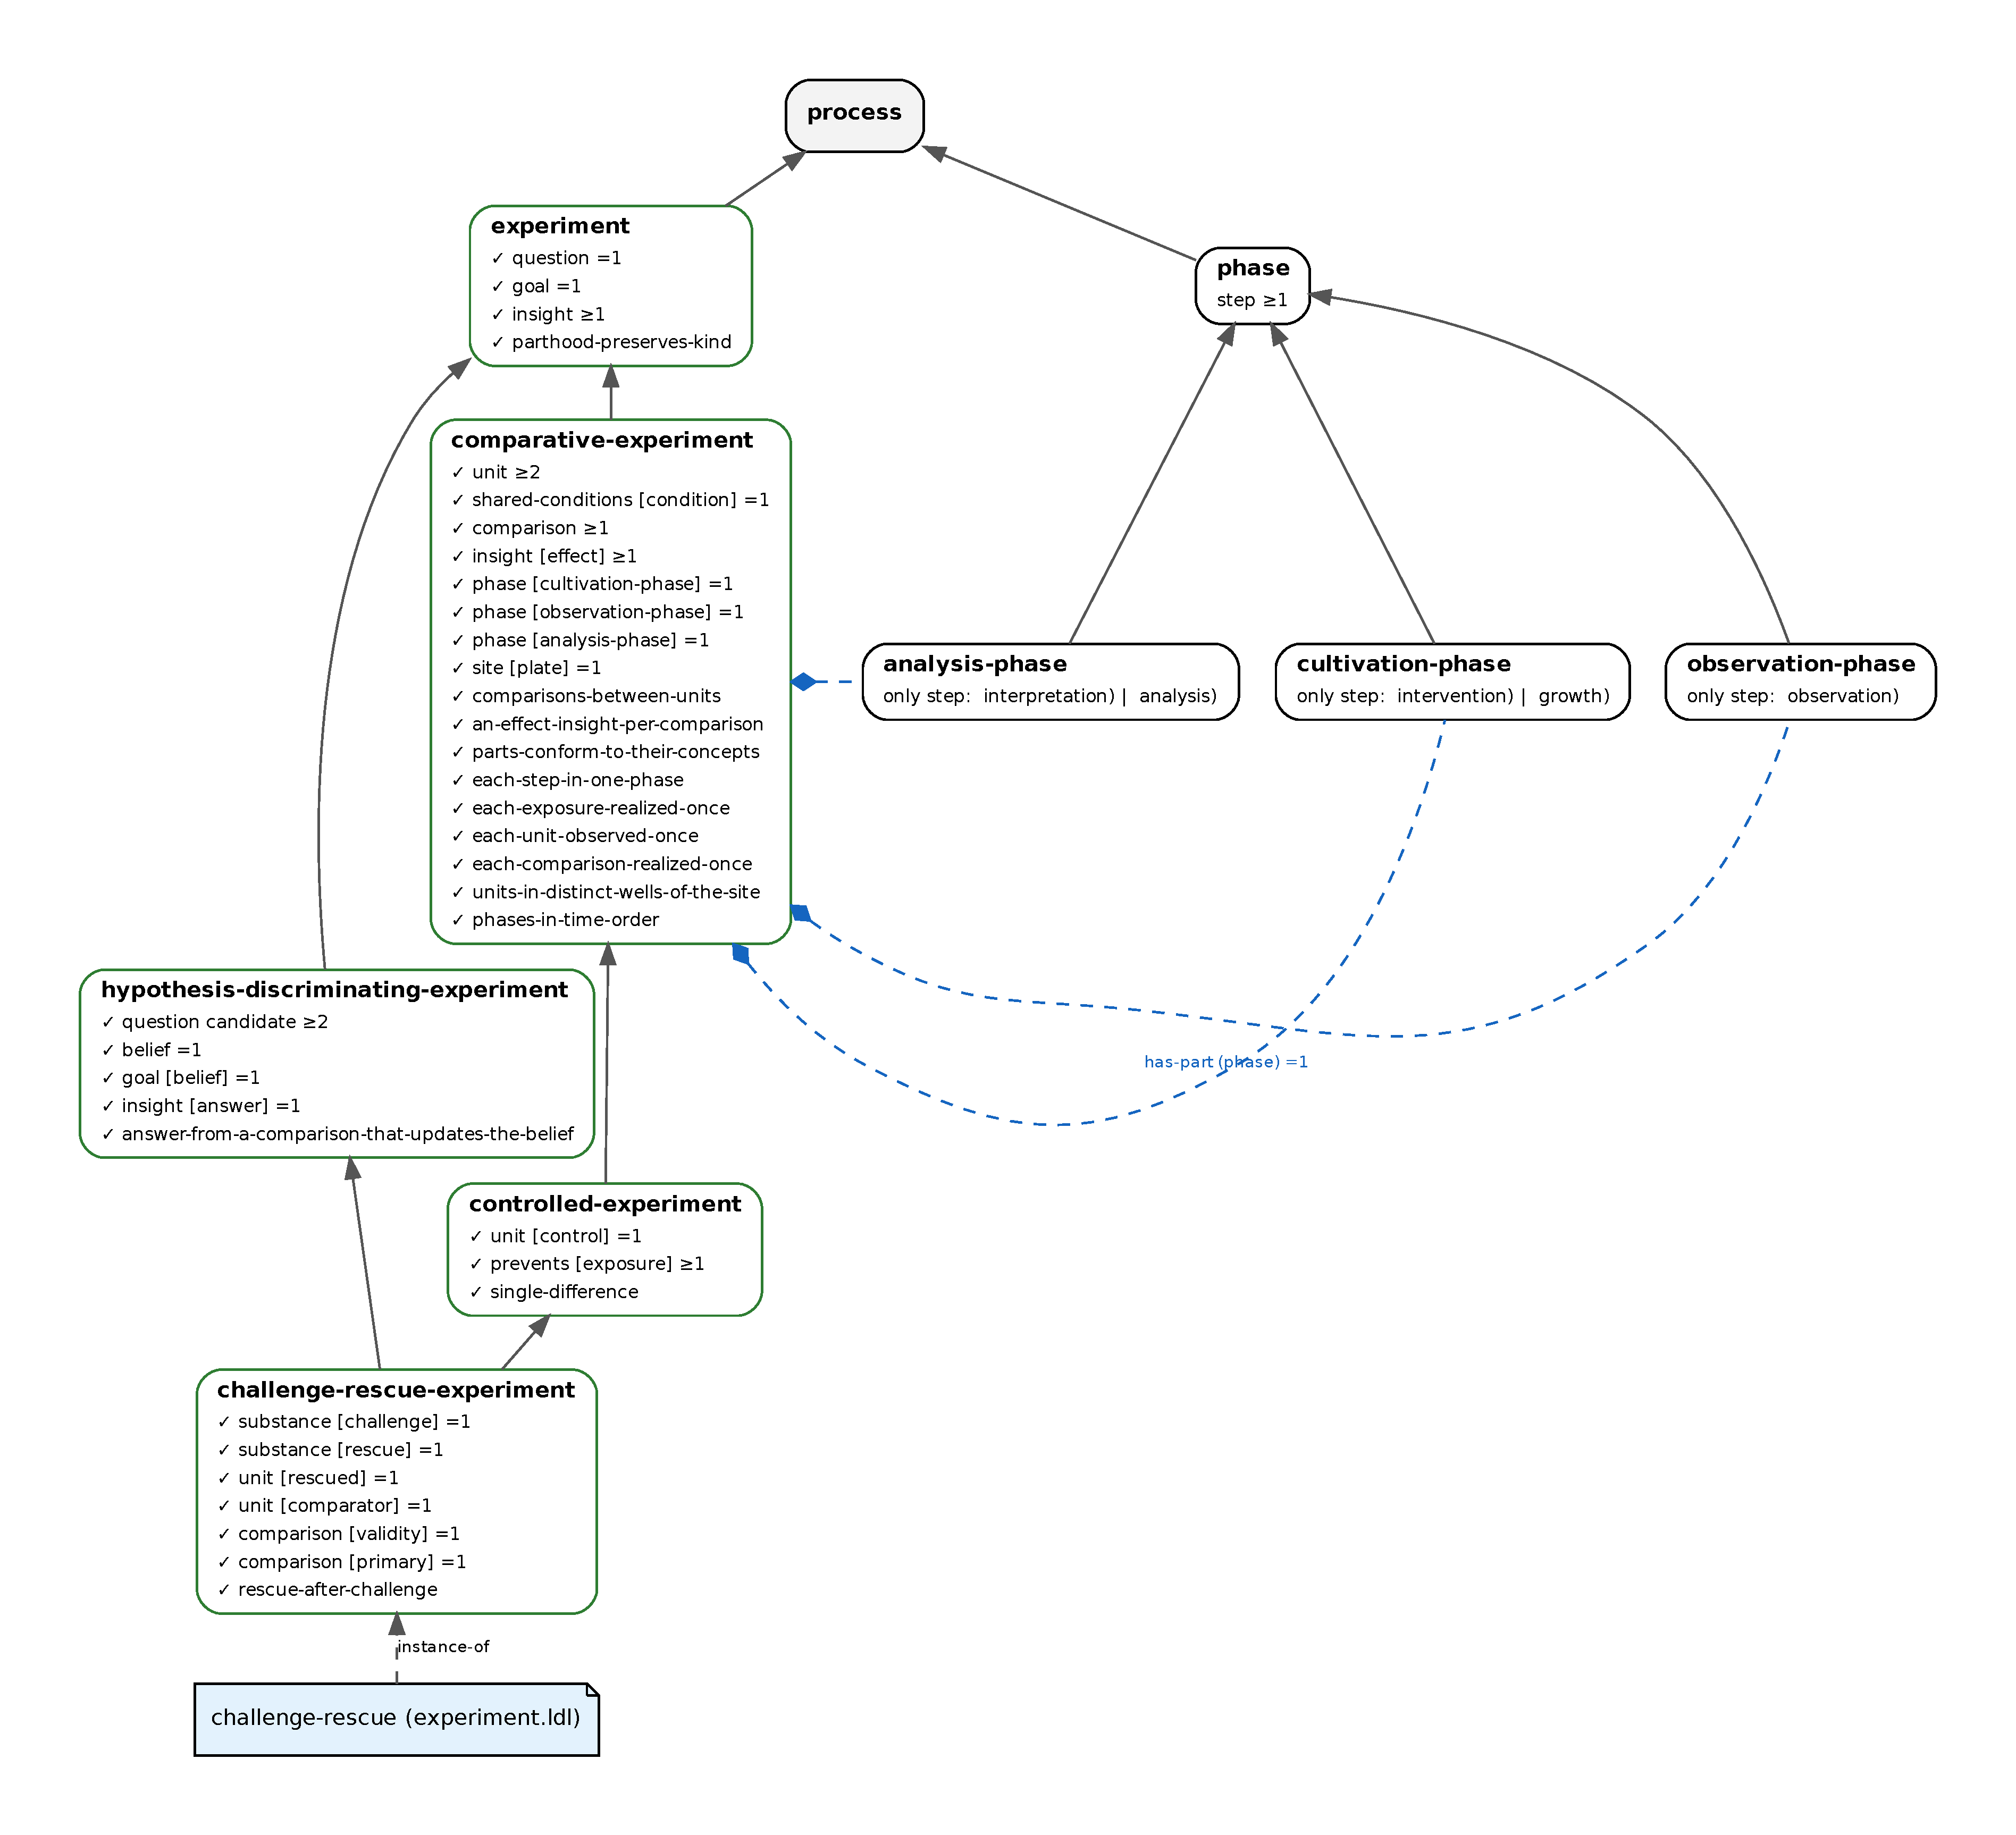
\includegraphics[width=\linewidth]{experiment_concepts.pdf}\end{center}
\subsection*{Experiment}an activity that answers a question by producing insights.
\ax{\mathsf{Experiment} ⊑ \mathsf{Process}}
\ax{\mathsf{Experiment} ⊑ (=1 \mathit{hasQuestion}.\mathsf{Question})}
\ax{\mathsf{Experiment} ⊑ (=1 \mathit{hasGoal}.⊤)}
\ax{\mathsf{Experiment} ⊑ ∃\mathit{hasInsight}.\mathsf{Insight}}
Further constraints (Section~\ref{sec:beyond}): \tth{parthood-\allowbreak{}preserves-\allowbreak{}kind}.
\subsection*{HypothesisDiscriminatingExperiment}the question asks which of several candidate hypotheses holds; the experiment changes a belief
over them, and its answer is the posterior.
\ax{\mathsf{HypothesisDiscriminatingExperiment} ⊑ \mathsf{Experiment}}
\ax{\mathsf{HypothesisDiscriminatingExperiment} ⊑ ∃\mathit{hasQuestion}.(≥2 \mathit{hasCandidate}.⊤)}
\ax{\mathsf{HypothesisDiscriminatingExperiment} ⊑ (=1 \mathit{hasBelief}.(\mathsf{Belief} ⊓\allowbreak ∃\mathit{over}.⊤ ⊓\allowbreak ∃\mathit{hasPrior}.⊤))}
\ax{\mathsf{HypothesisDiscriminatingExperiment} ⊑ (=1 \mathit{hasGoal}.(\mathsf{Belief} ⊓\allowbreak ∃\mathit{expectedInformationGain}.⊤))}
\ax{\mathsf{HypothesisDiscriminatingExperiment} ⊑ (=1 \mathit{hasInsight}.(\mathsf{Insight} ⊓\allowbreak ∃\mathit{hasRole}.\mathsf{AnswerRole} ⊓\allowbreak ∃\mathit{hasForm}.\mathsf{Posterior}))}
Further constraints (Section~\ref{sec:beyond}): \tth{answer-\allowbreak{}from-\allowbreak{}a-\allowbreak{}comparison-\allowbreak{}that-\allowbreak{}updates-\allowbreak{}the-\allowbreak{}belief}.
\subsection*{ComparativeExperiment}units are treated differently, kept under shared conditions and observed the same way;
comparisons between units determine the effects of the treatments. Its procedure yields three phases.
\ax{\mathsf{ComparativeExperiment} ⊑ \mathsf{Experiment}}
\ax{\mathsf{ComparativeExperiment} ⊑ (≥2 \mathit{hasUnit}.∃\mathit{hasTreatment}.⊤)}
\ax{\mathsf{ComparativeExperiment} ⊑ (=1 \mathit{hasSharedConditions}.(\mathsf{Condition} ⊓\allowbreak ∃\mathit{fromTime}.⊤ ⊓\allowbreak ∃\mathit{toTime}.⊤ ⊓\allowbreak ∃\mathit{hasObservation}.(\mathsf{Observation} ⊓\allowbreak ∃\mathit{atTime}.⊤ ⊓\allowbreak ∃\mathit{interpretedAs}.⊤)))}
\ax{\mathsf{ComparativeExperiment} ⊑ ∃\mathit{hasComparison}.(\mathsf{Comparison} ⊓\allowbreak ∃\mathit{between}.⊤ ⊓\allowbreak ∃\mathit{determines}.\mathsf{Effect})}
\ax{\mathsf{ComparativeExperiment} ⊑ ∃\mathit{hasInsight}.(\mathsf{Insight} ⊓\allowbreak ∃\mathit{hasRole}.\mathsf{EffectRole})}
\ax{\mathsf{ComparativeExperiment} ⊑ (=1 \mathit{hasPhase}.\mathsf{CultivationPhase})}
\ax{\mathsf{ComparativeExperiment} ⊑ (=1 \mathit{hasPhase}.\mathsf{ObservationPhase})}
\ax{\mathsf{ComparativeExperiment} ⊑ (=1 \mathit{hasPhase}.\mathsf{AnalysisPhase})}
\ax{\mathsf{ComparativeExperiment} ⊑ (=1 \mathit{hasSite}.\mathsf{Plate})}
Further constraints (Section~\ref{sec:beyond}): \tth{comparisons-\allowbreak{}between-\allowbreak{}units}, \tth{an-\allowbreak{}effect-\allowbreak{}insight-\allowbreak{}per-\allowbreak{}comparison}, \tth{parts-\allowbreak{}conform-\allowbreak{}to-\allowbreak{}their-\allowbreak{}concepts}, \tth{each-\allowbreak{}step-\allowbreak{}in-\allowbreak{}one-\allowbreak{}phase}, \tth{each-\allowbreak{}exposure-\allowbreak{}realized-\allowbreak{}once}, \tth{each-\allowbreak{}unit-\allowbreak{}observed-\allowbreak{}once}, \tth{each-\allowbreak{}comparison-\allowbreak{}realized-\allowbreak{}once}, \tth{units-\allowbreak{}in-\allowbreak{}distinct-\allowbreak{}wells-\allowbreak{}of-\allowbreak{}the-\allowbreak{}site}, \tth{phases-\allowbreak{}in-\allowbreak{}time-\allowbreak{}order}.
Procedure (rules that derive the actions; not DL axioms):\begin{itemize}[nosep,leftmargin=1.5em]\item {\small\tth{(rule (each exposure (of (a unit))) (yields (an action (kind intervention) (in (the cultivation-\allowbreak{}phase)))))}}\item {\small\tth{(rule (each interval (between (consecutive treatment-\allowbreak{}times))) (yields (an action (kind growth) (in (the cultivation-\allowbreak{}phase)))))}}\item {\small\tth{(rule (each unit) (yields (an action (kind observation) (in (the observation-\allowbreak{}phase))) (an action (kind interpretation) (in (the analysis-\allowbreak{}phase)))))}}\item {\small\tth{(rule (each comparison) (yields (an action (kind analysis) (in (the analysis-\allowbreak{}phase)))))}}\item {\small\tth{(rule (a comparison (licenses ?c)) (orders (its analysis) (before (the analysis (of ?c)))))}}\end{itemize}
\subsection*{ControlledExperiment}one unit is an untreated control, it stays untreated, and every comparison isolates exactly one
exposure: its two units differ in that exposure only, and it is the exposure whose effect the comparison determines.
\ax{\mathsf{ControlledExperiment} ⊑ \mathsf{ComparativeExperiment}}
\ax{\mathsf{ControlledExperiment} ⊑ (=1 \mathit{hasUnit}.(∃\mathit{hasRole}.\mathsf{ControlRole} ⊓\allowbreak ∃\mathit{hasTreatment}.\mathsf{EmptyTreatment}))}
\ax{\mathsf{ControlledExperiment} ⊑ ∃\mathit{prevents}.(\mathsf{Exposure} ⊓\allowbreak ∃\mathit{of}.(\mathsf{Culture} ⊓\allowbreak ∃\mathit{hasRole}.\mathsf{ControlRole}))}
Further constraints (Section~\ref{sec:beyond}): \tth{single-\allowbreak{}difference}.
\subsection*{ChallengeRescueExperiment}units are injured by a challenge; one is then given a rescue after a delay. A validity comparison
(comparator vs control) establishes the challenge's effect and licenses the primary comparison (rescued vs
comparator), which determines the rescue's effect and updates the belief over models of recovery.
\ax{\mathsf{ChallengeRescueExperiment} ⊑ \mathsf{ControlledExperiment} ⊓\allowbreak \mathsf{HypothesisDiscriminatingExperiment}}
\ax{\mathsf{ChallengeRescueExperiment} ⊑ (=1 \mathit{hasSubstance}.(\mathsf{Substance} ⊓\allowbreak ∃\mathit{hasRole}.\mathsf{ChallengeRole}))}
\ax{\mathsf{ChallengeRescueExperiment} ⊑ (=1 \mathit{hasSubstance}.(\mathsf{Substance} ⊓\allowbreak ∃\mathit{hasRole}.\mathsf{RescueRole}))}
\ax{\mathsf{ChallengeRescueExperiment} ⊑ (=1 \mathit{hasUnit}.(\mathsf{Culture} ⊓\allowbreak ∃\mathit{hasRole}.\mathsf{RescuedRole} ⊓\allowbreak ∃\mathit{hasTreatment}.(\mathsf{Treatment} ⊓\allowbreak ∃\mathit{hasExposure}.(\mathsf{Exposure} ⊓\allowbreak ∃\mathit{exposedTo}.(\mathsf{Substance} ⊓\allowbreak ∃\mathit{hasRole}.\mathsf{ChallengeRole})) ⊓\allowbreak ∃\mathit{hasExposure}.(\mathsf{Exposure} ⊓\allowbreak ∃\mathit{exposedTo}.(\mathsf{Substance} ⊓\allowbreak ∃\mathit{hasRole}.\mathsf{RescueRole})))))}
\ax{\mathsf{ChallengeRescueExperiment} ⊑ (=1 \mathit{hasUnit}.(\mathsf{Culture} ⊓\allowbreak ∃\mathit{hasRole}.\mathsf{ComparatorRole} ⊓\allowbreak ∃\mathit{hasTreatment}.(\mathsf{Treatment} ⊓\allowbreak ∃\mathit{hasExposure}.(\mathsf{Exposure} ⊓\allowbreak ∃\mathit{exposedTo}.(\mathsf{Substance} ⊓\allowbreak ∃\mathit{hasRole}.\mathsf{ChallengeRole})))))}
\ax{\mathsf{ChallengeRescueExperiment} ⊑ (=1 \mathit{hasComparison}.(\mathsf{Comparison} ⊓\allowbreak ∃\mathit{hasRole}.\mathsf{ValidityRole} ⊓\allowbreak ∃\mathit{between}.(\mathsf{Culture} ⊓\allowbreak ∃\mathit{hasRole}.\mathsf{ComparatorRole}) ⊓\allowbreak ∃\mathit{between}.(\mathsf{Culture} ⊓\allowbreak ∃\mathit{hasRole}.\mathsf{ControlRole}) ⊓\allowbreak ∃\mathit{determines}.(\mathsf{Effect} ⊓\allowbreak ∃\mathit{of}.(\mathsf{Substance} ⊓\allowbreak ∃\mathit{hasRole}.\mathsf{ChallengeRole})) ⊓\allowbreak ∃\mathit{licenses}.(\mathsf{Comparison} ⊓\allowbreak ∃\mathit{hasRole}.\mathsf{PrimaryRole})))}
\ax{\mathsf{ChallengeRescueExperiment} ⊑ (=1 \mathit{hasComparison}.(\mathsf{Comparison} ⊓\allowbreak ∃\mathit{hasRole}.\mathsf{PrimaryRole} ⊓\allowbreak ∃\mathit{between}.(\mathsf{Culture} ⊓\allowbreak ∃\mathit{hasRole}.\mathsf{RescuedRole}) ⊓\allowbreak ∃\mathit{between}.(\mathsf{Culture} ⊓\allowbreak ∃\mathit{hasRole}.\mathsf{ComparatorRole}) ⊓\allowbreak ∃\mathit{determines}.(\mathsf{Effect} ⊓\allowbreak ∃\mathit{of}.(\mathsf{Substance} ⊓\allowbreak ∃\mathit{hasRole}.\mathsf{RescueRole})) ⊓\allowbreak ∃\mathit{updates}.\mathsf{Belief}))}
Further constraints (Section~\ref{sec:beyond}): \tth{rescue-\allowbreak{}after-\allowbreak{}challenge}.
\section{Constraints beyond the TBox axioms}\label{sec:beyond}
\begin{tabularx}{\linewidth}{@{}p{3.6cm}>{\raggedright\arraybackslash}p{2.4cm}>{\raggedright\arraybackslash}X@{}}\toprule constraint & logic & statement \\ \midrule
\tth{parthood-\allowbreak{}preserves-\allowbreak{}kind} & OWL 2 DL & $\mathsf{Process} ⊑ ∀\mathit{hasPart}.\mathsf{Process}$ \newline $\mathsf{MaterialEntity} ⊑ ∀\mathit{hasPart}.\mathsf{MaterialEntity}$ \newline $\mathsf{PlanSpecification} ⊑ ∀\mathit{hasPart}.\mathsf{PlanSpecification}$ \newline $\mathsf{InformationEntity} ⊑ ∀\mathit{hasPart}.\mathsf{InformationEntity}$ \newline {\footnotesize\itshape stated in the kinds section; parthood never crosses kinds} \\[3pt]
\tth{answer-\allowbreak{}from-\allowbreak{}a-\allowbreak{}comparison-\allowbreak{}that-\allowbreak{}updates-\allowbreak{}the-\allowbreak{}belief} & OWL 2 DL & $\mathsf{Insight} ⊓\allowbreak ∃\mathit{hasRole}.\mathsf{AnswerRole} ⊑ ∃\mathit{from}.(\mathsf{Comparison} ⊓\allowbreak ∃\mathit{updates}.\mathsf{Belief})$ \newline {\footnotesize\itshape that the comparison is one of the same experiment needs variable sharing (FOL)} \\[3pt]
\tth{comparisons-\allowbreak{}between-\allowbreak{}units} & SROIQ role inclusion & $\mathit{hasComparison} ∘ \mathit{between} ⊑ \mathit{hasUnit}$ \newline {\footnotesize\itshape read as an integrity constraint: under the open world an OWL reasoner would infer the unit, not report it} \\[3pt]
\tth{an-\allowbreak{}effect-\allowbreak{}insight-\allowbreak{}per-\allowbreak{}comparison} & FOL & $∀e,c. \mathit{hasComparison}(e,c) → ∃i. \mathit{hasInsight}(e,i) ∧\allowbreak \mathit{from}(i,c) ∧\allowbreak ∀s. (\mathit{determines}∘\mathit{of})(c,s) → \mathit{of}(i,s)$ \newline {\footnotesize\itshape OWL 2 states only $\mathsf{Comparison} ⊑ ∃\mathit{from}^{-}.(\mathsf{Insight} ⊓ ∃\mathit{hasRole}.\mathsf{EffectRole})$} \\[3pt]
\tth{parts-\allowbreak{}conform-\allowbreak{}to-\allowbreak{}their-\allowbreak{}concepts} & DL semantics & (every TBox axiom holds of every individual) \newline {\footnotesize\itshape the closed-world checker evaluates each part against its own concept} \\[3pt]
\tth{each-\allowbreak{}step-\allowbreak{}in-\allowbreak{}one-\allowbreak{}phase} & OWL 2 DL & $\mathsf{Action} ⊑ (=1 \mathit{hasStep}^{-}.\mathsf{Phase})$ \\[3pt]
\tth{each-\allowbreak{}exposure-\allowbreak{}realized-\allowbreak{}once} & OWL 2 DL + rule & $\mathsf{Exposure} ⊑ (=1 \mathit{realizes}^{-}.\mathsf{InterventionAction})$ \newline $realizes(a,x) ← \mathit{hasCulture}(a,u) ∧\allowbreak \mathit{hasTreatment}(u,t) ∧\allowbreak \mathit{hasExposure}(t,x) ∧\allowbreak \text{ same substance, dose and time}$ \newline {\footnotesize\itshape the rule that computes realizes compares data values of two individuals (SWRL)} \\[3pt]
\tth{each-\allowbreak{}unit-\allowbreak{}observed-\allowbreak{}once} & FOL & $∀e,u. \mathit{hasUnit}(e,u) → ∃^{=1} s. \mathit{hasPart}(e,s) ∧\allowbreak \mathsf{ObservationAction}(s) ∧\allowbreak \mathit{hasCulture}(s,u)$ \newline {\footnotesize\itshape OWL 2 states only $\mathsf{Culture} ⊑ (=1 \mathit{hasCulture}^{-}.\mathsf{ObservationAction})$, not 'within the same experiment'} \\[3pt]
\tth{each-\allowbreak{}comparison-\allowbreak{}realized-\allowbreak{}once} & OWL 2 DL + rule & $\mathsf{Comparison} ⊑ (=1 \mathit{realizes}^{-}.\mathsf{AnalysisAction})$ \newline {\footnotesize\itshape realizes is computed from the analysis's statistic (the pair of units it compares)} \\[3pt]
\tth{units-\allowbreak{}in-\allowbreak{}distinct-\allowbreak{}wells-\allowbreak{}of-\allowbreak{}the-\allowbreak{}site} & FOL (path agreement) & $\mathsf{Culture} ⊑ (=1 \mathit{containedIn}.\mathsf{Well}),   \mathsf{Well} ⊑ (≤1 \mathit{contains}.⊤)$ \newline $∀e,u,v. \mathit{hasUnit}(e,u) ∧\allowbreak \mathit{hasUnit}(e,v) → (\mathit{containedIn}∘\mathit{partOf})(u) = (\mathit{containedIn}∘\mathit{partOf})(v)$ \newline {\footnotesize\itshape the first line is OWL 2 DL; 'one plate for all units' is a role-value map, undecidable with the rest} \\[3pt]
\tth{phases-\allowbreak{}in-\allowbreak{}time-\allowbreak{}order} & ALC(D) feature chains & $\mathsf{ComparativeExperiment} ⊑ ∃(\mathit{cultivation}∘\mathit{toTime}, \mathit{observationPhase}∘\mathit{atTime}).≤$ \newline {\footnotesize\itshape compares two data values reached by different paths: a concrete-domain predicate, not available in OWL 2} \\[3pt]
\tth{single-\allowbreak{}difference} & FOL with counting & $∀c,u,v. \mathit{between}(c,u) ∧\allowbreak \mathit{between}(c,v) ∧\allowbreak u≠v → |X(u) △ X(v)| = 1 ∧\allowbreak ∀x ∈ X(u) △ X(v). \mathit{exposedTo}(x) = (\mathit{determines}∘\mathit{of})(c)$ \newline (X(u): the exposures of the treatment of u, as substance, dose and time) \newline {\footnotesize\itshape beyond SROIQ: compares two individuals' sets of exposures (rule with aggregation, SPARQL, or the checker)} \\[3pt]
\tth{rescue-\allowbreak{}after-\allowbreak{}challenge} & ALC(D) feature chains & $∃\mathit{hasRole}.\mathsf{RescuedRole} ⊑ ∃(\mathit{rescueExposure}∘\mathit{atTime}, \mathit{challengeExposure}∘\mathit{atTime}).>$ \newline {\footnotesize\itshape with rescueExposure, challengeExposure functional subroles of hasTreatment∘hasExposure; not OWL 2} \\[3pt]
\bottomrule\end{tabularx}
\section{The challenge-rescue experiment as an instance}
The ABox below is the experiment of \texttt{experiment.ldl} as derived (phases and steps from the procedure) and placed (plate and wells from the mapping to Cell~01). Doses and times are omitted.
\begin{center}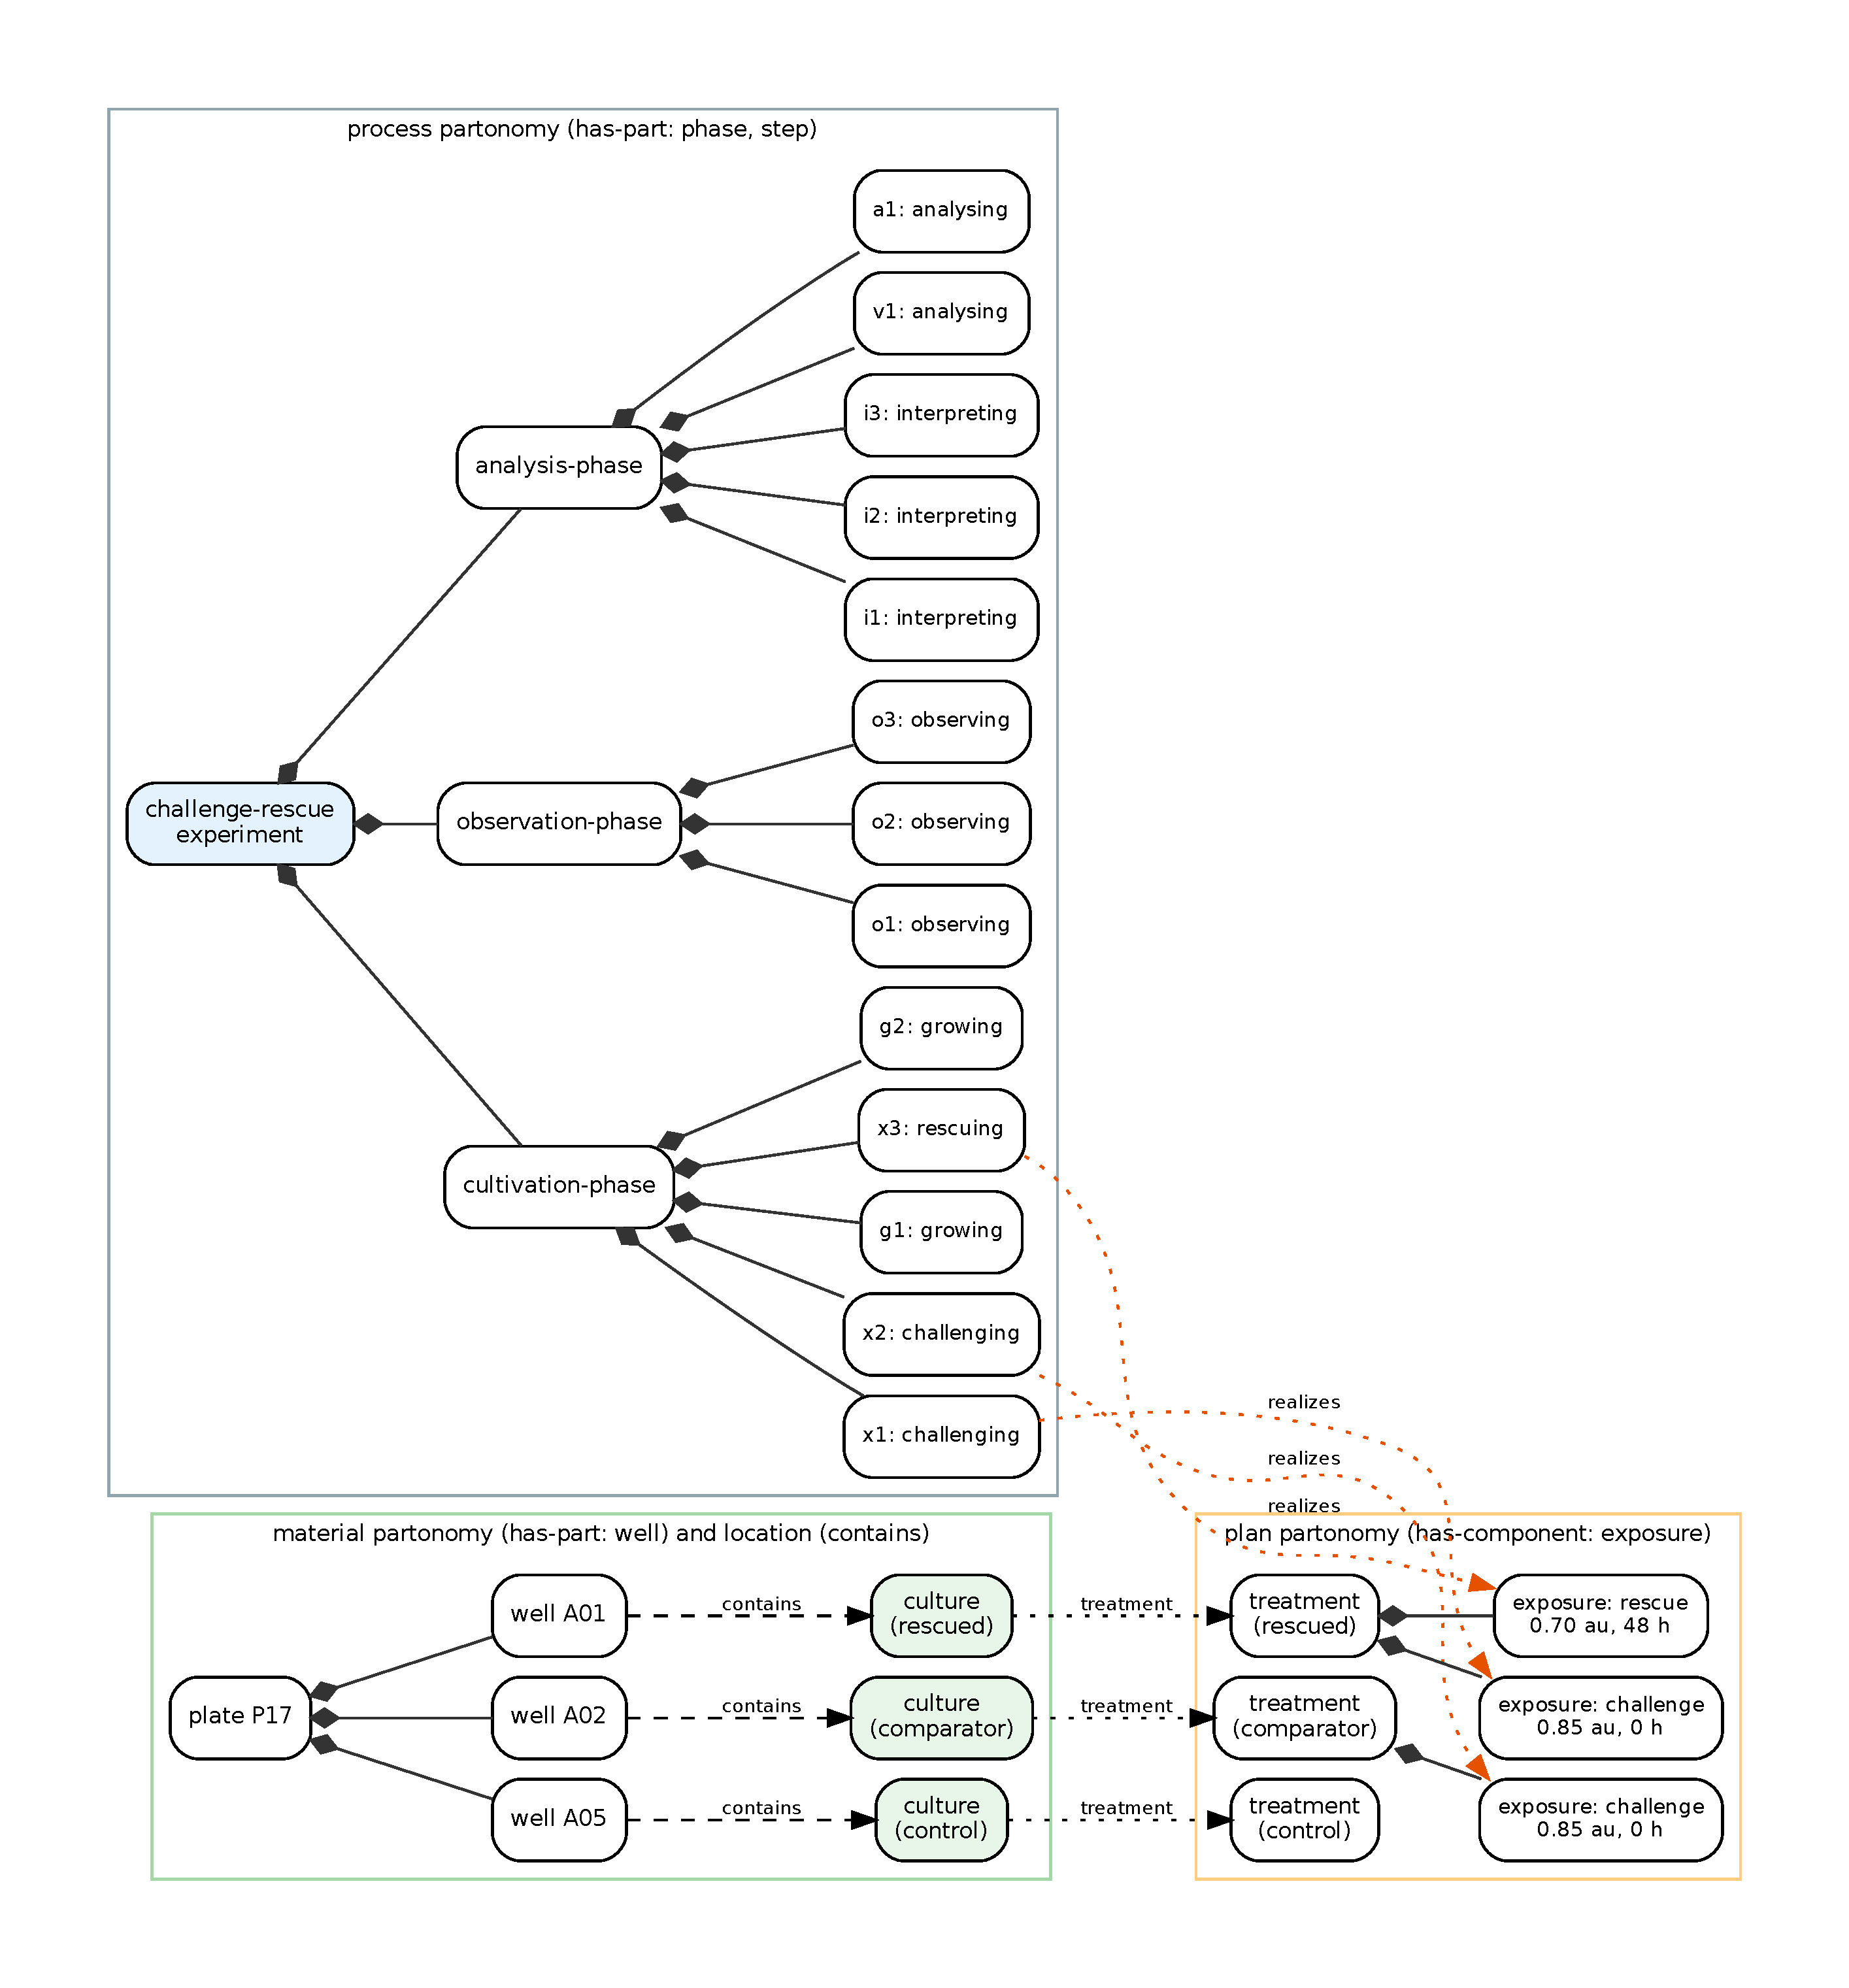
\includegraphics[width=\linewidth]{experiment_partonomy.pdf}\end{center}
{\small\begin{multicols}{2}
$\mathsf{ChallengeRescueExperiment}(\mathtt{e})$\par
$\mathit{hasQuestion}(\mathtt{e}, \mathtt{q})$\par
$\mathsf{RecoveryModel}(\mathtt{M1\_graded})$\par
$\mathit{hasCandidate}(\mathtt{q}, \mathtt{M1\_graded})$\par
$\mathsf{RecoveryModel}(\mathtt{M2\_threshold})$\par
$\mathit{hasCandidate}(\mathtt{q}, \mathtt{M2\_threshold})$\par
$\mathsf{RecoveryModel}(\mathtt{M3\_protective})$\par
$\mathit{hasCandidate}(\mathtt{q}, \mathtt{M3\_protective})$\par
$\mathsf{Belief}(\mathtt{b})$\par
$\mathit{hasBelief}(\mathtt{e}, \mathtt{b})$\par
$\mathsf{Substance}(\mathtt{s\_challenge})$\par
$\mathit{hasRole}(\mathtt{s\_challenge}, \mathtt{challengeRole})$\par
$\mathit{hasSubstance}(\mathtt{e}, \mathtt{s\_challenge})$\par
$\mathsf{Substance}(\mathtt{s\_rescue})$\par
$\mathit{hasRole}(\mathtt{s\_rescue}, \mathtt{rescueRole})$\par
$\mathit{hasSubstance}(\mathtt{e}, \mathtt{s\_rescue})$\par
$\mathsf{Culture}(\mathtt{rescued})$\par
$\mathit{hasCulture}(\mathtt{e}, \mathtt{rescued})$\par
$\mathit{hasRole}(\mathtt{rescued}, \mathtt{rescuedRole})$\par
$\mathsf{Treatment}(\mathtt{t\_rescued})$\par
$\mathit{hasTreatment}(\mathtt{rescued}, \mathtt{t\_rescued})$\par
$\mathsf{Exposure}(\mathtt{x\_rescued\_challenge})$\par
$\mathit{hasExposure}(\mathtt{t\_rescued}, \mathtt{x\_rescued\_challenge})$\par
$\mathit{exposedTo}(\mathtt{x\_rescued\_challenge}, \mathtt{s\_challenge})$\par
$\mathsf{Exposure}(\mathtt{x\_rescued\_rescue})$\par
$\mathit{hasExposure}(\mathtt{t\_rescued}, \mathtt{x\_rescued\_rescue})$\par
$\mathit{exposedTo}(\mathtt{x\_rescued\_rescue}, \mathtt{s\_rescue})$\par
$\mathsf{Culture}(\mathtt{comparator})$\par
$\mathit{hasCulture}(\mathtt{e}, \mathtt{comparator})$\par
$\mathit{hasRole}(\mathtt{comparator}, \mathtt{comparatorRole})$\par
$\mathsf{Treatment}(\mathtt{t\_comparator})$\par
$\mathit{hasTreatment}(\mathtt{comparator}, \mathtt{t\_comparator})$\par
$\mathsf{Exposure}(\mathtt{x\_comparator\_challenge})$\par
$\mathit{hasExposure}(\mathtt{t\_comparator}, \mathtt{x\_comparator\_challenge})$\par
$\mathit{exposedTo}(\mathtt{x\_comparator\_challenge}, \mathtt{s\_challenge})$\par
$\mathsf{Culture}(\mathtt{control})$\par
$\mathit{hasCulture}(\mathtt{e}, \mathtt{control})$\par
$\mathit{hasRole}(\mathtt{control}, \mathtt{controlRole})$\par
$\mathsf{EmptyTreatment}(\mathtt{t\_control})$\par
$\mathit{hasTreatment}(\mathtt{control}, \mathtt{t\_control})$\par
$\mathsf{Comparison}(\mathtt{c\_validity})$\par
$\mathit{hasComparison}(\mathtt{e}, \mathtt{c\_validity})$\par
$\mathit{between}(\mathtt{c\_validity}, \mathtt{comparator})$\par
$\mathit{between}(\mathtt{c\_validity}, \mathtt{control})$\par
$\mathit{licenses}(\mathtt{c\_validity}, \mathtt{c\_primary})$\par
$\mathsf{Comparison}(\mathtt{c\_primary})$\par
$\mathit{hasComparison}(\mathtt{e}, \mathtt{c\_primary})$\par
$\mathit{between}(\mathtt{c\_primary}, \mathtt{rescued})$\par
$\mathit{between}(\mathtt{c\_primary}, \mathtt{comparator})$\par
$\mathsf{Insight}(\mathtt{ins\_answer})$\par
$\mathit{hasInsight}(\mathtt{e}, \mathtt{ins\_answer})$\par
$\mathit{from}(\mathtt{ins\_answer}, \mathtt{c\_primary})$\par
$\mathsf{Insight}(\mathtt{ins\_effect\_rescue})$\par
$\mathit{hasInsight}(\mathtt{e}, \mathtt{ins\_effect\_rescue})$\par
$\mathit{from}(\mathtt{ins\_effect\_rescue}, \mathtt{c\_primary})$\par
$\mathsf{Insight}(\mathtt{ins\_effect\_challenge})$\par
$\mathit{hasInsight}(\mathtt{e}, \mathtt{ins\_effect\_challenge})$\par
$\mathit{from}(\mathtt{ins\_effect\_challenge}, \mathtt{c\_validity})$\par
$\mathsf{CultivationPhase}(\mathtt{cultivation})$\par
$\mathit{hasPhase}(\mathtt{e}, \mathtt{cultivation})$\par
$\mathsf{InterventionAction}(\mathtt{x1})$\par
$\mathit{hasStep}(\mathtt{cultivation}, \mathtt{x1})$\par
$\mathsf{InterventionAction}(\mathtt{x2})$\par
$\mathit{hasStep}(\mathtt{cultivation}, \mathtt{x2})$\par
$\mathsf{GrowthAction}(\mathtt{g1})$\par
$\mathit{hasStep}(\mathtt{cultivation}, \mathtt{g1})$\par
$\mathsf{InterventionAction}(\mathtt{x3})$\par
$\mathit{hasStep}(\mathtt{cultivation}, \mathtt{x3})$\par
$\mathsf{GrowthAction}(\mathtt{g2})$\par
$\mathit{hasStep}(\mathtt{cultivation}, \mathtt{g2})$\par
$\mathsf{ObservationPhase}(\mathtt{observation})$\par
$\mathit{hasPhase}(\mathtt{e}, \mathtt{observation})$\par
$\mathsf{ObservationAction}(\mathtt{o1})$\par
$\mathit{hasStep}(\mathtt{observation}, \mathtt{o1})$\par
$\mathsf{ObservationAction}(\mathtt{o2})$\par
$\mathit{hasStep}(\mathtt{observation}, \mathtt{o2})$\par
$\mathsf{ObservationAction}(\mathtt{o3})$\par
$\mathit{hasStep}(\mathtt{observation}, \mathtt{o3})$\par
$\mathsf{AnalysisPhase}(\mathtt{analysis})$\par
$\mathit{hasPhase}(\mathtt{e}, \mathtt{analysis})$\par
$\mathsf{InterpretationAction}(\mathtt{i1})$\par
$\mathit{hasStep}(\mathtt{analysis}, \mathtt{i1})$\par
$\mathsf{InterpretationAction}(\mathtt{i2})$\par
$\mathit{hasStep}(\mathtt{analysis}, \mathtt{i2})$\par
$\mathsf{InterpretationAction}(\mathtt{i3})$\par
$\mathit{hasStep}(\mathtt{analysis}, \mathtt{i3})$\par
$\mathsf{AnalysisAction}(\mathtt{v1})$\par
$\mathit{hasStep}(\mathtt{analysis}, \mathtt{v1})$\par
$\mathsf{AnalysisAction}(\mathtt{a1})$\par
$\mathit{hasStep}(\mathtt{analysis}, \mathtt{a1})$\par
$\mathit{realizes}(\mathtt{x1}, \mathtt{x\_rescued\_challenge})$\par
$\mathit{realizes}(\mathtt{x2}, \mathtt{x\_comparator\_challenge})$\par
$\mathit{realizes}(\mathtt{x3}, \mathtt{x\_rescued\_rescue})$\par
$\mathit{realizes}(\mathtt{v1}, \mathtt{c\_validity})$\par
$\mathit{realizes}(\mathtt{a1}, \mathtt{c\_primary})$\par
$\mathsf{Plate}(\mathtt{P17})$\par
$\mathit{hasSite}(\mathtt{e}, \mathtt{P17})$\par
$\mathsf{Well}(\mathtt{A01})$\par
$\mathit{hasWell}(\mathtt{P17}, \mathtt{A01})$\par
$\mathit{contains}(\mathtt{A01}, \mathtt{rescued})$\par
$\mathsf{Well}(\mathtt{A02})$\par
$\mathit{hasWell}(\mathtt{P17}, \mathtt{A02})$\par
$\mathit{contains}(\mathtt{A02}, \mathtt{comparator})$\par
$\mathsf{Well}(\mathtt{A05})$\par
$\mathit{hasWell}(\mathtt{P17}, \mathtt{A05})$\par
$\mathit{contains}(\mathtt{A05}, \mathtt{control})$\par
\end{multicols}}
\subsection*{Conformance and classification (closed world)}
\begin{tabular}{@{}lrr@{}}\toprule concept & constraints & satisfied \\ \midrule
Experiment & 4 & 4 \\
ComparativeExperiment & 17 & 17 \\
ControlledExperiment & 3 & 3 \\
HypothesisDiscriminatingExperiment & 5 & 5 \\
ChallengeRescueExperiment & 7 & 7 \\
\bottomrule\end{tabular}
\par Most specific concept: $\mathsf{ChallengeRescueExperiment}$ (declared: $\mathsf{ChallengeRescueExperiment}$). Every part satisfies its own concept (50/50).
\subsection*{Negative controls}
\begin{tabularx}{\linewidth}{@{}>{\raggedright\arraybackslash}p{4.6cm}>{\raggedright\arraybackslash}X>{\raggedright\arraybackslash}X@{}}\toprule modification & fails at & still an instance of \\ \midrule
comparator dose 0.60 au & ControlledExperiment & HypothesisDiscriminatingExperiment, ComparativeExperiment \\
control culture removed & ComparativeExperiment, ControlledExperiment & HypothesisDiscriminatingExperiment \\
rescue given with the challenge (0 h) & ChallengeRescueExperiment & HypothesisDiscriminatingExperiment, ControlledExperiment \\
belief and answer removed & HypothesisDiscriminatingExperiment & ControlledExperiment \\
rescue intervention missing from the plan & ComparativeExperiment & HypothesisDiscriminatingExperiment \\
comparator on another plate & ComparativeExperiment & HypothesisDiscriminatingExperiment \\
an observation step in two phases & ComparativeExperiment & HypothesisDiscriminatingExperiment \\
a well as part of a treatment & Experiment, ComparativeExperiment & --- \\
\bottomrule\end{tabularx}
\end{document}